\documentclass[11pt]{article}

% parameters are fairly self-explanatory here, thankfully
\usepackage[width=7in,height=9.5in,top=0.75in,centering]{geometry}

% for math-ing
\usepackage{amsmath}
\usepackage{amssymb}
\usepackage{comment}

%%%%%% tables %%%%%%%%

\usepackage{array}
\renewcommand{\arraystretch}{1.5}
\setlength{\tabcolsep}{8pt}

%%%%%% plotting %%%%%%

\usepackage[dvipsnames]{xcolor}
\usepackage{tikz}
\usepackage{pgfplots}

\pgfplotsset{every axis/.append style={
                    axis x line=middle,    % put the x axis in the middle
                    axis y line=middle,    % put the y axis in the middle
                    axis line style={<->,color=black}, % arrows on the axis
                    xlabel={$x$},          % default put x on x-axis
                    ylabel={$y$},          % default put y on y-axis
            }}
            
 \pgfplotsset{compat=1.14} % sometimes, everything falls apart without this
 
 %\usepgfplotslibrary{fillbetween} %for shading between curves

%%%%%% commands %%%%%%

% exam heading; course name is first argument, exam information is second argument
\newcommand{\Heading}[2]{
    \fbox{
        {\Large\textbf{#1}}
        }
    \hfill
    \fbox{
        \begin{minipage}{0.2\textwidth}
            \begin{center}
            \textbf{#2}
            \end{center}
        \end{minipage}
    }
    \par\vspace{0.1in}}

% for being lazy while beautifying integrals
\newcommand{\dint}{\displaystyle\int}

% for being lazy while beautifying limits
\newcommand{\dlim}{\displaystyle\lim}

%%%%%% stuff %%%%%%

\usepackage{fancyhdr}

%\setcounter{page}{0} % first page is page 0

\parindent0pt % no indent

\fboxsep=0.25cm % little space in fbox border

%%%%%% BEGIN! %%%%%%%

\begin{document}

\pagestyle{fancy}

% record goals here to create sense of transparency

\fancyhead[c]{%
  \ifcase\value{page}
  % empty test for page = 0
  \or {}% 
  \or
  \or {\bf\color{ProcessBlue} F1: Lines \& Slope}% page=1
  \or {\bf\color{RoyalBlue} L1: Limits and Continuity}% page = 2
  \or {\bf\color{RoyalBlue} L2: Evaluating Limits Using Continuity and Forms}% page = 3
  \or {\bf\color{ForestGreen} D1: Meaning of a Derivative}% page = 4
  \or {\bf\color{ProcessBlue} F2: Exponential and Logarithmic Functions}% page = 5
  \or {\bf\color{ForestGreen} D3: Derivatives of Basic Functions}% page = 7
  \or {\bf\color{ForestGreen} D2: Compute Derivatives}% page = 6
  \or {\bf\color{RedOrange} A1: Derivatives and Graphing}% page = 8
  \or
  \else
  % Empty chead here!
  \fi
}

\thispagestyle{empty} % don't display that this is page 0

\Heading{MATH 1190/1210 Survey of Calculus I}{Knowledge Checkpoint 2\\Spring 2026}

\vspace{0.1in}

\textbf{Name} \hrulefill \, \begin{minipage}{0.16\textwidth}\begin{center}\textbf{UVA ID\\ (e.g. hdj4nd)} \end{center}\end{minipage}\hrulefill\\

\begin{minipage}{0.2\textwidth}\begin{center}\textbf{Course \&\\ Section Number} \end{center}\end{minipage} \hrulefill\,\,\textbf{Date} \hrulefill  \\

\hrulefill
\paragraph*{Course \& Section Numbers:}

{\small
\begin{center}
\begin{tabular}{| c | c | c | c |}
\hline
\begin{minipage}{0.12\textwidth}\centering
1190-100\\
J. Rolf\\
(2:00 PM)
\end{minipage}
&
\begin{minipage}{0.12\textwidth}\centering
1190-200\\
J. Rolf\\
(3:30 PM)
\end{minipage}
&
\begin{minipage}{0.12\textwidth}\centering
1190-300\\
Michael\\
(11 AM)
\end{minipage}
&
\begin{minipage}{0.12\textwidth}\centering
1210-200\\
Susan\\
(9:30 AM)
\end{minipage}
\\ \hline
\begin{minipage}{0.12\textwidth}\centering
1210-300\\
Susan\\
(2 PM)
\end{minipage}
&
\begin{minipage}{0.12\textwidth}\centering
1210-400\\
Holden\\
(12:30 PM)
\end{minipage}
&
\begin{minipage}{0.12\textwidth}\centering
1210-500\\
Susan\\
(3:30 PM)
\end{minipage}
&
\begin{minipage}{0.12\textwidth}\centering
1210-700\\
Aaratrick\\
(2:00 PM)
\end{minipage}
\\ \hline
\begin{minipage}{0.12\textwidth}\centering
1210-800\\
J. Bowling\\
(3:30 PM)
\end{minipage}
&
\begin{minipage}{0.12\textwidth}\centering
1210-900\\
J. Bowling\\
(5 PM)
\end{minipage}
&
\begin{minipage}{0.12\textwidth}\centering
1210-930\\
Vadim\\
(11 AM)
\end{minipage}
\\
\cline{1-3}
\end{tabular}
\end{center}
}


{%\small

\paragraph*{Instructions:}

\begin{itemize}
    
    \item The regular time allowed for completing this assessment is \fbox{$80$} minutes.
    %\item This assessment is out of 50 points.\\
    \item This assessment contains one single-part or multi-part problem for each of the following targets: {\bf\color{ProcessBlue}F1}, {\bf\color{RoyalBlue}L1}, {\bf\color{RoyalBlue}L2}, {\bf\color{ForestGreen}D1}, {\bf\color{ProcessBlue}F2}, {\bf\color{ForestGreen}D3}, {\bf\color{ForestGreen}D2}, {\bf\color{RedOrange}A1}.
    \item On each problem, you will receive a score of Exceeds Expectations (5), Proficient (4), Almost (3), Developing (2), Emerging (1), or Not Yet (0). {\bf Please do not interpret your score as a percentage.}
    %\item You will have opportunities to reassess on the targets appearing on this assessment after the next {\bf 2} assessments.\\
    \item You may NOT use calculators, dictionaries, notes, phones, or any other kind of aid.
    \item Please write neatly. What cannot be read, cannot be graded.
    \item Carefully work out each problem and clearly indicate your final answer to every problem.
    \item Throughout, give the most descriptive answer possible. \textbf{For instance, ``DNE" will not be accepted when ``$=\infty$" is applicable.}
    %\item Please provide the most specific answer possible. For instance, if a limit does not exist because it goes to $\infty$ or $-\infty$, then specify this.
    \item Please use the methods discussed up to this point in the course. For example, any work based on l'H\^opital's Rule will not receive credit.
    \item \textbf{All work must be shown unless otherwise specified.} Partial credit will not be given if appropriate work is not shown.
    \item In particular, {\bf any answer appearing with no justification will receive no credit regardless of whether the answer was correct}, unless otherwise specified.
    \item Please first respond to the prompts on which you feel most proficient, then respond to others later.
    \item This booklet is printed double-sided. It contains 12 pages and 8 numbered problems.
    \end{itemize}
    
    }

\vfill


%%%%%%%%%
\newpage

This page is left blank intentionally.\\

Use this page if you need additional space to write your solutions to any problem. \\

If you wish this page graded, you must refer to this page on \textbf{the original page} of the problem. Otherwise, your grader will NOT consider your work on this page.

\newpage%
%%%%%%%%%


\begin{enumerate}

%%%%%%%%%%%%%%%%%%%%%%%%%%%%%%%%%%%%%%%%%%%%%%%%%%%%%
%%%%%%%%%%% BEGIN PROBLEM F1 %%%%%%%%%%%%%%%%%%%%%%%%
%%%%%%%%%%%%%%%%%%%%%%%%%%%%%%%%%%%%%%%%%%%%%%%%%%%%%

\item Abe is taking a road trip on I-81 to see his father, who lives 160 miles away. 
He plans a stop at his sister Beth's house, who live 75 miles away. The graph below models Abe's trip:

\begin{center}
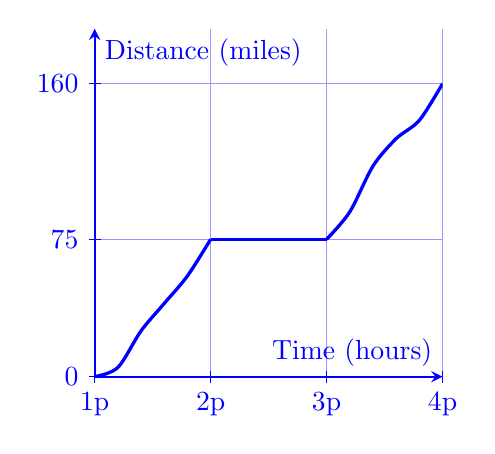
\begin{tikzpicture}
\begin{axis}[
    width=6cm,
    height=6cm,
    xmin=12, xmax=15,
    ymin=0, ymax=190,
    xtick={12,13,14,15},
    xticklabels={1p,2p,3p,4p},
    ytick={0,75,160},
    xlabel={Time (hours)},
    ylabel={Distance (miles)},
    axis lines=left,
    grid=both,
    major grid style={blue!40},
    minor grid style={blue!20},
    tick style={blue},
    label style={blue},
    tick label style={blue},
    axis line style={blue},
    thick
]

% First segment (varying speed)
\addplot[blue, very thick, smooth] 
coordinates {
(12,0)
(12.2,5)
(12.4,25)
(12.6,40)
(12.8,55)
(13,75)
};

% Stopped segment
\addplot[blue, very thick] coordinates {(13,75) (14,75)};

% Final segment (varying speed again)
\addplot[blue, very thick, smooth] 
coordinates {
(14,75)
(14.2,90)
(14.4,115)
(14.6,130)
(14.8,140)
(15,160)
};
\end{axis}
\end{tikzpicture}
\end{center}






Abe leaves at 1{:}00\,PM and 
Abe arrives at Beth's house at 2{:}00\,PM, stays until 3{:}00\,PM and arrives at his father's house at 4{:}00\,PM.

\bigskip

\begin{enumerate}
    \item Calculate the net change in Abe's distance between 2{:}00\,PM and 4{:}00\,PM and include all units.
    {\color{blue}\[160-75=85\]}
        \,\hfill units: {\color{blue}miles}\\
    
    \item Calculate the average rate of change (AROC) of Abe's distance driven between 1{:}00\,PM and 4{:}00\,PM and include all units.\\

   {\color{blue}\[\frac{160-0}{4-1}=\frac{160}{3}=53.333\]}
        \,\hfill units: {\color{blue}miles per hour}\\
    \item Use a sentence or two to explain the meaning of this average rate of change
    \textbf{in the context of this scenario}. 
    \begin{center}
    {\color{blue}Abe's average speed is 53.33 miles per hour.}
    \end{center}

\end{enumerate}

%%%%%%%%%%%%%%%%%%%%%%%%%%%%%%%%%%%%%%%%%%%%%%%%%%%%%
%%%%%%%%%%% END PROBLEM F1 %%%%%%%%%%%%%%%%%%%%%%%%%%
%%%%%%%%%%%%%%%%%%%%%%%%%%%%%%%%%%%%%%%%%%%%%%%%%%%%%

\newpage

%%%%%%%%%%%%%%%%%%%%%%%%%%%%%%%%%%%%%%%%%%%%%%%%%%%%%
%%%%%%%%%%% BEGIN PROBLEM L1 %%%%%%%%%%%%%%%%%%%%%%%%
%%%%%%%%%%%%%%%%%%%%%%%%%%%%%%%%%%%%%%%%%%%%%%%%%%%%%
\item Use the three answer choices -- A, B, and C -- given below to respond to the prompts that follow. If none of these answer choices is correct, then write ``n/a".\\
\begin{comment}
\begin{tabular}{l l}
\fbox{A} &
\begin{tabular}{| c || c c c c c c c |}
\hline
$x$  & $0.9$ & $0.99$ & $0.999$ & $1$ & $1.001$ & $1.01$ & $1.1$\\ 
\hline
$y$ & $2.8$ & $2.95$  & $2.99$ & $3$ & $3.01$ & $3.05$  & $3.2$\\
\hline
\end{tabular}\\[0.25in]

\fbox{B} &
\begin{tabular}{| c || c c c c c c c |}
\hline
$x$  & $0.9$ & $0.99$ & $0.999$ & $1$ & $1.001$ & $1.01$ & $1.1$\\ 
\hline
$y$ & $2.8$ & $2.95$  & $2.99$ & $-1$ & $-1.01$ & $-1.05$  & $-1.2$\\
\hline
\end{tabular}\\[0.25in]

\fbox{C} &
\begin{tabular}{| c || c |c |c |c |c |c |c |}
\hline
$x$  & $0.9$ & $0.99$ & $0.999$ & $1$ & $1.001$ & $1.01$ & $1.1$\\ 
\hline
$y$ & $2.8$ & $2.95$  & $2.99$ & undefined & $3.01$ & $3.05$  & $3.2$\\
\hline
\end{tabular}
\end{tabular}
\bigskip
\end{comment}
\begin{tabular}{l l l}
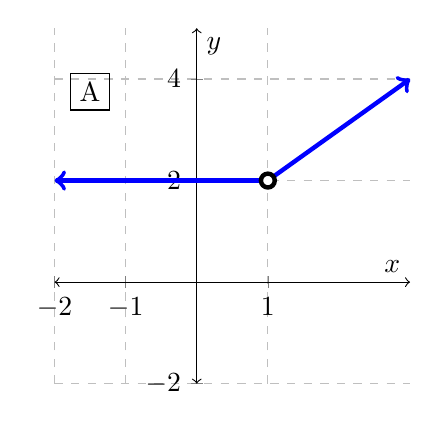
\begin{tikzpicture}[scale=1]
\begin{axis}[
xlabel={$x$},
xtick = {-2,-1,1},
xticklabels = {$-2$,$-1$,$1$},
ylabel={$y$},
ytick = {-2,2,4},
yticklabels = {$-2$,$2$,$4$},
samples=160,
domain=-1:3,
xmin=-2, xmax=3,
ymin=-2, ymax=5,
grid=both, grid style=dashed,
width=2.4in, height=2.4in
]
\addplot[ultra thick,blue,<-,domain=-2:1] {2};
\addplot[ultra thick,blue,->,domain=1:3] {x+1};
\filldraw[fill=white,ultra thick] (1,2) circle (2.5pt);
\node at (-1.5,3.75){\fbox{A}};
\end{axis}
\end{tikzpicture}
&
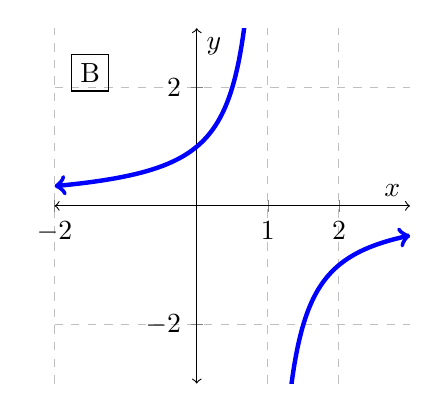
\begin{tikzpicture}[scale=1]
\begin{axis}[
xlabel={$x$},
xtick = {-2,1,2},
xticklabels = {$-2$,$1$,$2$},
ylabel={$y$},
ytick = {-2,2},
yticklabels = {$-2$,$2$},
samples=160,
domain=-1:3,
xmin=-2, xmax=3,
ymin=-3, ymax=3,
grid=both, grid style=dashed,
width=2.4in, height=2.4in
]
\addplot[ultra thick,blue,<->,domain=-2:0.99] {-1/(x-1)};
\addplot[ultra thick,blue,<->,domain=1.01:3] {-1/(x-1)};
\node at (-1.5,2.25) {\fbox{B}};
\end{axis}
\end{tikzpicture}
&
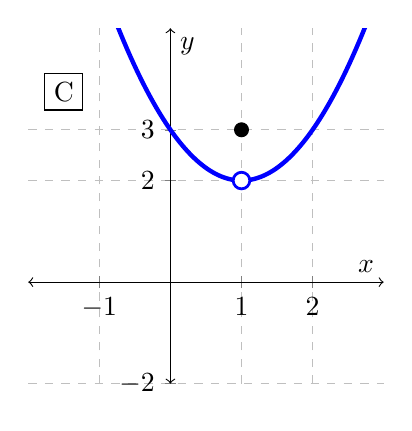
\begin{tikzpicture}[scale=1]
\begin{axis}[
xlabel={$x$},
xtick = {-1,1,2},
xticklabels = {$-1$,$1$,$2$},
ylabel={$y$},
ytick = {-2,2,3},
yticklabels = {$-2$,$2$,$3$},
samples=160,
domain=-1:3,
xmin=-2, xmax=3,
ymin=-2, ymax=5,
grid=both, grid style=dashed,
width=2.4in, height=2.4in
]
\addplot[ultra thick,blue,<->,domain=-1:3] {(x-1)^2+2};
\filldraw (1,3) circle (2.5pt);
\node at (-1.5,3.75) {\fbox{C}};
\addplot[
    only marks,
    mark=*,
    mark size=3pt,
    mark options={
        draw=blue,
        line width=1pt,
        fill=white
    }
]
coordinates {(1,2)};
\end{axis}
\end{tikzpicture}
\\
\end{tabular}

\bigskip
\hfill {\bf Write all correct answer choices.} \hfill \\



\begin{minipage}[t]{0.48\textwidth}
\begin{enumerate}
\item[(a)] Which of the answer choices describes a function $f$ for which 
\[
\lim_{x\to1}f(x) \text{ DNE?}
\]
\end{enumerate}

\,\hfill Answer (a):
\rule[-8pt]{1in}{0.4pt}{\color{blue} B}\rule[-8pt]{1in}{0.4pt} \\
\end{minipage}
%
\hfill
%
\begin{minipage}[t]{0.48\textwidth}
\begin{enumerate}
\item[(b)] Which of the answer choices describes a function $g$ for which 
\[
\lim_{x\to1}g(x)=2?
\]
\end{enumerate}

\,\hfill Answer (b):
\rule[-8pt]{1in}{0.2pt}{\color{blue} A, C}\rule[-8pt]{1in}{0.2pt} \\
\end{minipage}

\vspace{2cm}  % space between rows

\begin{minipage}[t]{0.48\textwidth}
\begin{enumerate}
\item[(c)] Which of the answer choices describe a function so that $\displaystyle \lim_{x\to1}f(x)$ does exist, but $f(1)$ does not exist?
\end{enumerate}

\,\hfill Answer (c):
\rule[-8pt]{1in}{0.4pt}{\color{blue} A}\rule[-8pt]{1in}{0.4pt} \\
\end{minipage}
%
\hfill
%
\begin{minipage}[t]{0.48\textwidth}
\begin{enumerate}
\item[(d)] Which of the answer choices describe a continuous function?\\
\end{enumerate}

\,\hfill Answer (d):
\rule[-8pt]{1in}{0.3pt}{\color{blue} n/a}\rule[-8pt]{1in}{0.3pt} \\
\end{minipage}
\newpage

%%%%%%%%%%%%%%%%%%%%%%%%%%%%%%%%%%%%%%%%%%%%%%%%%%%%%
%%%%%%%%%%% END PROBLEM L1 %%%%%%%%%%%%%%%%%%%%%%%%%%
%%%%%%%%%%%%%%%%%%%%%%%%%%%%%%%%%%%%%%%%%%%%%%%%%%%%%

%%%%%%%%%%%%%%%%%%%%%%%%%%%%%%%%%%%%%%%%%%%%%%%%%%%%%
%%%%%%%%%%% BEGIN PROBLEM L2 %%%%%%%%%%%%%%%%%%%%%%%%
%%%%%%%%%%%%%%%%%%%%%%%%%%%%%%%%%%%%%%%%%%%%%%%%%%%%%
\item For each limit below, first determine the form of the limit, then find the value of the limit. 
If the given function is continuous at the target, you may simply write ``n/a'' for the form. 
Show complete work --- using mathematics and/or words --- to justify your answers. 
({\it Note:} $e \approx 2.718$.)


\begin{enumerate}
    \item[(a)] $\displaystyle\lim_{x\to\infty} \frac{3x^2 + e^{2x}}{\ln(x) - 5}$
    \hspace{1cm}
    \textbf{form:} {\color{blue} $\frac{\infty}{\infty}$ } \quad
    \textbf{value:} {\color{blue} $\infty$}
    \smallskip

    {\color{blue}
    Both the numerator and denominator grow without bound as $x \to \infty$, so the form is $\frac\infty\infty$. The dominant terms are $e^{2x}$ and $\ln x$ in the numerator and denominator respectively. Since exponentials grow much faster that logarithms, we get the value of the limit is $\infty$.
    }
\bigskip

    \item[(b)] 
    $\displaystyle\lim_{x\to0} \frac{e^{3x} + 1 - 3x}{\ln(x + 2)}$
    \hspace{1cm}
    \textbf{form:} {\color{blue} N/A or $\frac{c}{c}$} \quad
    \textbf{value:} {\color{blue} $\frac{2}{\ln(2)}$}
    \smallskip

    {\color{blue}
    The function $\frac{e^{3x} + 1 - 3x}{\ln(x + 2)}$ is defined at $x=0$, and is hence continuous at that point by the Main Continuity Theorem. Therefore, the limit can be evaluated by plugging in $x=0$ in the function, which gives $\frac{2}{\ln(2)}$.
    }
    \bigskip

    \item[(c)] 
    $\displaystyle\lim_{x\to 0^{+}} \frac{\sqrt{4x + 5} - x^3}{2x^3 + \ln(x)}$
    \hspace{1cm}
    \textbf{form:} {\color{blue} $\frac{c}{\infty}$} \quad
    \textbf{value:} {\color{blue} 0}
    \smallskip

    {\color{blue}
    As $x \to 0^+$, the numerator approaches 5 using continuity, and the denominator approaches $-\infty$ because $2x^3$ approaches 0 and $\ln x$ approaches $-\infty$. This means the form is $\frac{c}{\infty}$ and the value is hence 0.
    }
\end{enumerate}
%%%%%%%%%%%%%%%%%%%%%%%%%%%%%%%%%%%%%%%%%%%%%%%%%%%%%
%%%%%%%%%%% END PROBLEM L2 %%%%%%%%%%%%%%%%%%%%%%%%%%
%%%%%%%%%%%%%%%%%%%%%%%%%%%%%%%%%%%%%%%%%%%%%%%%%%%%%

\newpage

%%%%%%%%%%%%%%%%%%%%%%%%%%%%%%%%%%%%%%%%%%%%%%%%%%%%%
%%%%%%%%%%% BEGIN PROBLEM D1 %%%%%%%%%%%%%%%%%%%%%%%%
%%%%%%%%%%%%%%%%%%%%%%%%%%%%%%%%%%%%%%%%%%%%%%%%%%%%%
\item {\bf You may simply write your answers with no justification on this problem.}

\begin{enumerate}
    \item The pressure $P$ (in psi) inside a sealed container depends on the temperature $T$ (in ${}^{\circ}\!C$). In general, as temperature increases, the pressure increases.
    \begin{enumerate}
        \item In terms of the context above, what does $P'(50)$ represent? What are its units?

    \vspace{1cm}
    {\color{blue}The instantaneous rate at which pressure is changing with respect to temperature when the temperature is $50^\circ C$.}

        \,\hfill units in i.: {\color{blue}psi/$^\circ$C}
    

        \item In terms of the context above, what does 
        \[
        \frac{P(80)-P(40)}{80-40}
        \]
        represent? What are its units?
        
    \vspace{1cm}
     {\color{blue}The average rate of change of pressure with respect to temperature between $40^\circ C$ and $80^\circ C$.}
    
        \,\hfill units in ii.: {\color{blue}psi/$^\circ$C}
        
    \end{enumerate}

    \item[(b)] The graph of a function $g$ is given below.
\end{enumerate}

\begin{minipage}[t][2.75in][t]{0.35\textwidth}
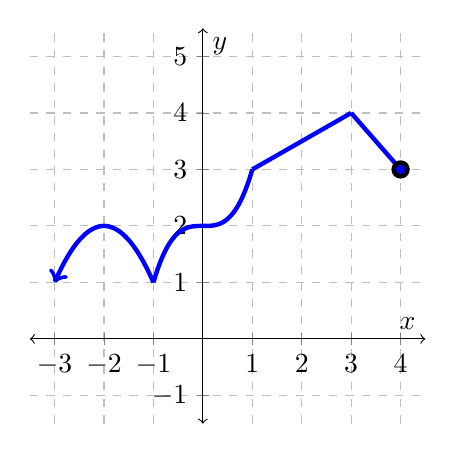
\begin{tikzpicture}[scale=1]
\begin{axis}[
xlabel={$x$},
ylabel={$y$},
xtick={-3,-2,-1,1,2,3,4},
ytick={-1,1,2,3,4,5},
samples=300,
domain=-3:4.5,
xmin=-3.5, xmax=4.5,
ymin=-1.5, ymax=5.5,
width=2.6in, height=2.6in,
grid=both, grid style=dashed
]

% left curve
\addplot[domain=-3:-1, blue, ultra thick,<-] {2-(x+2)^2};

% middle smooth curve
\addplot[domain=-1:1, blue, ultra thick] {x^3+2};

% line segment
\draw[blue, ultra thick] (1,3) -- (3,4);

% ray to right
\draw[blue, ultra thick] (3,4) -- (4,3);

% open circle
\filldraw[ultra thick, fill=blue] (4,3) circle (2.5pt);

\end{axis}
\end{tikzpicture}
\end{minipage}
%%%%%%%%%%%%%%%%%
\begin{minipage}[t][2.75in][t]{0.6\textwidth}
\begin{enumerate}
    \item[i.] List all $x$ values for which $g'(x)$ DNE: 

    \hfill $x=$ {\color{blue}$-1,\;1,\;3,\;4$}


    \item[ii.] Mark the boxes in the table below to indicate what can be said about the given quantities.
\end{enumerate}

\vspace{-0.1in}

\begin{tabular}{m{2.4in} m{0.6in} m{0.6in} m{0.6in}}
 & positive? & negative? & zero?\\[0.1in]

$\bullet$ $\displaystyle\lim_{x\to 2}\frac{g(x)-g(2)}{x-2}$ is $\dotfill$ 
& {\color{blue}$\blacksquare$} & $\square$ & $\square$ \\[0.2in]

$\bullet$ $\displaystyle\frac{g(4)-g(3)}{4-3}$ is $\dotfill$ 
& $\square$ & {\color{blue}$\blacksquare$} & $\square$ \\[0.2in]

$\bullet$ $g'(-2)$ is $\dotfill$ 
& $\square$ & $\square$ & {\color{blue}$\blacksquare$} \\

\end{tabular}
\end{minipage}

%%%%%%%%%%%%%%%%%%%%%%%%%%%%%%%%%%%%%%%%%%%%%%%%%%%%%
%%%%%%%%%%% END PROBLEM D1 %%%%%%%%%%%%%%%%%%%%%%%%%%
%%%%%%%%%%%%%%%%%%%%%%%%%%%%%%%%%%%%%%%%%%%%%%%%%%%%%

\newpage

%%%%%%%%%%%%%%%%%%%%%%%%%%%%%%%%%%%%%%%%%%%%%%%%%%%%%
%%%%%%%%%%% BEGIN PROBLEM F2 %%%%%%%%%%%%%%%%%%%%%%%%
%%%%%%%%%%%%%%%%%%%%%%%%%%%%%%%%%%%%%%%%%%%%%%%%%%%%%

\item Respond to the following prompts. For this specific question, you are not required to compute any powers of constants or logarithms. For example, if your final answer includes $10^3$ or $\log_2(5)$, you can leave it as is.

\begin{enumerate}
    \item Simplify the expression below as much as possible so that the final result contains only positive exponents. You may expand exponential expressions and/or apply properties of exponents as needed. 

    \[\left(\dfrac{2 \ x^{-1/2}y^{-3}}{3\ xy^{-1}}\right)^2\]
    {\color{blue}\[\left(\dfrac{2 \ x^{-1/2}y^{-3}}{3\ xy^{-1}}\right)^2=\dfrac{2^2 \ (x^{-1/2})^2(y^{-3})^2}{3^2\ x^2(y^{-1})^2}=\dfrac{2^2 \ x^{-1}y^{-6}}{3^2\ x^2y^{-2}}=\dfrac{2^2 \ (y^{2})}{3^2\ x^2(y^{6})(x^1)}=\dfrac{2^2 \ y^2}{3^2\ x^3y^6}=\dfrac{2^2}{3^2\ x^3y^4}\text{ or }\dfrac{4}{9\ x^3y^4}\]}
    
    \vfill

    \item Solve the following equation for $x$. 

    \[\log_{3}(x) + \log_{3}(x - 8) = 2\]

    {\color{blue}\[\log_{3}\left(x(x-8)\right)=2\]
    \[3^{\log_{3}(x(x-8))}=3^2\]
    \[x(x-8)=3^2\]
    \[x^2-8x=3^2\]
    \[x^2-8x=9\]
    \[x^2-8x-9=0\]
    \[(x-9)(x+1)=0\]
    Our potential solutions are $x=9$ and $x=-1$. However $x=-1$ cannot be a solution to the original equation since $\log_{3}(-1)$ and $\log_{3}(-1-8)$ are undefined.\\
    Final answer: $x=9$}

    \vfill
     \item Solve the following equation for $x$. 

    \[9^{2x - 1} = 81^{2x}\]


    {\color{blue}\begin{center}
        \[\log_{9}(9^{2x-1})=\log_{9}(81^{2x})\]
        \[(2x-1)\log_{9}(9)=(2x)\log_{9}(81)\]
        \[(2x-1)\log_{9}(9^1)=(2x)\log_{9}(9^2)\]
        \[(2x-1)(1)=(2x)(2)\]
        \[2x-1=4x\]
        \[-1=2x\]
        \[x=\frac{-1}{2}\]
    \end{center}}

    \vfill
\end{enumerate}


%%%%%%%%%%%%%%%%%%%%%%%%%%%%%%%%%%%%%%%%%%%%%%%%%%%%%
%%%%%%%%%%% END PROBLEM F2 %%%%%%%%%%%%%%%%%%%%%%%%%%
%%%%%%%%%%%%%%%%%%%%%%%%%%%%%%%%%%%%%%%%%%%%%%%%%%%%%

\newpage

%%%%%%%%%%%%%%%%%%%%%%%%%%%%%%%%%%%%%%%%%%%%%%%%%%%%%
%%%%%%%%%%% BEGIN PROBLEM D3 %%%%%%%%%%%%%%%%%%%%%%%%
%%%%%%%%%%%%%%%%%%%%%%%%%%%%%%%%%%%%%%%%%%%%%%%%%%%%%

\item Write down the derivatives of the following functions. No work required. No need to simplify.

If you need to write down your work, please do so at the bottom half of this page, not in the answer space.

\begin{center}
        \begin{tabular}{l c c l c c}
            %
            $\displaystyle\frac{d}{dx}\left[ 3x^{7} \right]$ & $=$ & $\overset{\displaystyle{\color{blue} 21x^6}}{\rule[-8pt]{1.5in}{0.4pt}}$ &
            %
            $\displaystyle\frac{d}{dx}\left[ \dfrac{1}{\sqrt[4]{x^5}} \right]$ & $=$ & $\overset{\displaystyle{\color{blue} -\frac{5}{4}x^{-9/4}}}{\rule[-8pt]{1.5in}{0.4pt}}$\\[4cm]

            %%%%%
            $\displaystyle\frac{d}{dx}\left[ \left(\dfrac{1}{2}\right)^x \right]$ & $=$ & $\overset{\displaystyle{\color{blue} \left(\frac{1}{2}\right)^x\ln\left(\frac{1}{2}\right)}}{\rule[-8pt]{1.5in}{0.4pt}}$ & 
            %%%%%
            $\displaystyle\frac{d}{dx}\left[ e^{\pi} \right]$ & $=$ & $\overset{\displaystyle{\color{blue} 0}}{\rule[-8pt]{1.5in}{0.4pt}}$\\[4cm]
            %%%%%
            $\displaystyle\frac{d}{dx}\left[ x^2+1 \right]$ & $=$ & $\overset{\displaystyle{\color{blue} 2x}}{\rule[-8pt]{1.5in}{0.4pt}}$&
            %
            $\displaystyle\frac{d}{dx}\left[ \sqrt[3]{x}-\ln(x) \right]$ & $=$ & $\overset{\displaystyle{\color{blue} \frac{1}{3}x^{-2/3} - \frac{1}{x}}}{\rule[-8pt]{1.5in}{0.4pt}}$\\[4cm]
            %%%%%
            $\displaystyle\frac{d}{dx}\left[ \dfrac{x^4+x^2-x}{x^4} \right]$ & $=$ & $\overset{\displaystyle{\color{blue} -2x^{-3} + 3x^{-4}}}{\rule[-8pt]{1.5in}{0.4pt}}$ & 
            %
            $\displaystyle\frac{d}{dx}\left[ \log_{3}(x) \right]$ & $=$ & $\overset{\displaystyle{\color{blue} \frac{1}{x\ln(3)}}}{\rule[-8pt]{1.5in}{0.4pt}}$
            %%%%%
        \end{tabular}
\end{center}
\hspace{1cm}\begin{minipage}{0.4\textwidth}
    {\color{blue} This answer was obtained by simplifying before taking the derivative with the power rule. One could instead apply the quotient rule directly to get
    \[
        \frac{x^4(4x^3+2x-1) - (x^4+x^2-x)(4x^3)}{(x^4)^2}.
    \]
    }
\end{minipage}


%%%%%%%%%%%%%%%%%%%%%%%%%%%%%%%%%%%%%%%%%%%%%%%%%%%%%
%%%%%%%%%%% END PROBLEM D3 %%%%%%%%%%%%%%%%%%%%%%%%%%
%%%%%%%%%%%%%%%%%%%%%%%%%%%%%%%%%%%%%%%%%%%%%%%%%%%%%

\newpage

%%%%%%%%%%%%%%%%%%%%%%%%%%%%%%%%%%%%%%%%%%%%%%%%%%%%%
%%%%%%%%%%% BEGIN PROBLEM D2 %%%%%%%%%%%%%%%%%%%%%%%%
%%%%%%%%%%%%%%%%%%%%%%%%%%%%%%%%%%%%%%%%%%%%%%%%%%%%%

\item Find the derivative of the following expressions. 

A correct final answer receives full credit. Nevertheless, you are encouraged to write down the steps so that you will be able to receive partial credit if you final answer is not fully correct. There's no need to simplify your final answer.

\begin{enumerate}
\item $\dfrac{(x^2 - 2x +2)e^x}{x^3}$

\medskip

{\color{blue}
Let \( f(x) = (x^2-2x+2)e^x \) and \( g(x) = x^3 \). Using the product rule, and then the sum rule, power rule and derivative of \( e^x \), we get
\[
    f'(x) = (2x-2)e^x + (x^2-2x+2)e^x = x^2e^x,
\]
and using the power rule, \( g'(x) = 3x^2 \). Using the quotient rule, we get
\[
    \frac{\textrm{d}}{\textrm{d}x} \left[\frac{(x^2-2x+2)e^x}{x^3}\right] = \frac{g(x)f'(x)-f(x)g'(x)}{g(x)^2} = \frac{x^3 \left((2x-2)e^x+(x^2-2x+2)e^x\right) - 3x^2(x^2-2x+2)e^x}{x^6},
\]
or using the simplified \( f'(x) \),
\[
    \frac{\textrm{d}}{\textrm{d}x} \left[\frac{(x^2-2x+2)e^x}{x^3}\right] = \frac{x^5e^x - 3x^2(x^2-2x+2)e^x}{x^6}.
\]
}

\bigskip

\item $\log_{2}(x)\left(4x+x^2\right)^5$

\medskip

{
\color{blue}
Let \( f(x) = (4x+x^2)^5 \). Using the chain rule with inner function \( 4x+x^2 \) and outer function \( x^5 \), we get
\[
    f'(x) = 5(4x+x^2)^4(4+2x),
\]
where we use the power rule and the sum rule to compute the derivatives of the inner and outer functions. Using the product rule
\[
    \frac{\textrm{d}}{\textrm{d}x}\left[\log_2(x) (4x+x^2)^5\right] = \frac{(4x+x^2)^5}{x \ln 2}+ 5 \log_2(x)(4x+x^2)^4(4+2x),
\]
where we also use the derivative of the general logarithmic function.
}
\end{enumerate}

%split part (a) and part (b)

%%%%%%%%%%%%%%%%%%%%%%%%%%%%%%%%%%%%%%%%%%%%%%%%%%%%%
%%%%%%%%%%% END PROBLEM D2 %%%%%%%%%%%%%%%%%%%%%%%%%%
%%%%%%%%%%%%%%%%%%%%%%%%%%%%%%%%%%%%%%%%%%%%%%%%%%%%%

\newpage

%%%%%%%%%%%%%%%%%%%%%%%%%%%%%%%%%%%%%%%%%%%%%%%%%%%%%
%%%%%%%%%%% BEGIN PROBLEM A1 %%%%%%%%%%%%%%%%%%%%%%%%
%%%%%%%%%%%%%%%%%%%%%%%%%%%%%%%%%%%%%%%%%%%%%%%%%%%%%

\item Consider the following function $f(x)$.

\[f(x)=x + \frac{1}{x}\]

Respond to the following prompts. Make sure to show all work.

\begin{enumerate}
    \item Find all critical numbers of $f(x)$.

    {\color{blue}
    \[
    f'(x)=1-\frac{1}{x^2}
    \]

    Critical numbers occur when $f'(x)=0$ or undefined (and $x$ is in the domain).

    \[
    1-\frac{1}{x^2}=0
    \]

    \[
    1=\frac{1}{x^2}
    \]

    \[
    x^2=1
    \]

    \[
    x=\pm1
    \]

    Since $x=0$ is not in the domain of $f(x)$, it is not a critical number.

    \[
    \textbf{Critical numbers: } x=-1,\;1
    \]
    }

    \item On what interval(s) is $f(x)$ concave up? On what intervals(s) is $f(x)$ concave down?

 {\color{blue}

    \[
    f''(x)=\frac{2}{x^3}
    \]

    The second derivative is undefined at $x=0$.

    \vspace{0.3cm}

    \textbf{Sign chart for $f''(x)$:}

    \[
    \begin{array}{c|ccc}
    x & (-\infty,0) & 0 & (0,\infty)\\
    \hline
    f''(x) & - & \text{undefined} & +
    \end{array}
    \]

    \vspace{0.3cm}

    Concave down when $f''(x)<0$:

    \[
    (-\infty,0)
    \]

    Concave up when $f''(x)>0$:

    \[
    (0,\infty)
    \]

    }
    \item Find all inflection points of $f(x)$.

 {\color{blue}

    Inflection points occur where concavity changes and the function is defined.

    Although concavity changes at $x=0$, the function is not defined there.

    Therefore,

    \[
    \textbf{There are no inflection points.}
    \]

    }
\end{enumerate}




%%%%%%%%%%%%%%%%%%%%%%%%%%%%%%%%%%%%%%%%%%%%%%%%%%%%%
%%%%%%%%%%% END PROBLEM A1 %%%%%%%%%%%%%%%%%%%%%%%%%%
%%%%%%%%%%%%%%%%%%%%%%%%%%%%%%%%%%%%%%%%%%%%%%%%%%%%%

\newpage

This page is left blank intentionally.\\

Use this page if you need additional space to write your solutions to any problem. \\

If you wish this page graded, you must refer to this page on \textbf{the original page} of the problem. Otherwise, your grader will NOT consider your work on this page.

\newpage

This page is left blank intentionally.\\

Use this page if you need additional space to write your solutions to any problem. \\

If you wish this page graded, you must refer to this page on \textbf{the original page} of the problem. Otherwise, your grader will NOT consider your work on this page.

\end{enumerate}

\end{document}